% diagrams/english/salon.tex -- el salón de los Brown, para "Where is
% it?": el sofá, la mesita baja (con sitio debajo), el sillón, la
% ventana y una lámpara de pie.
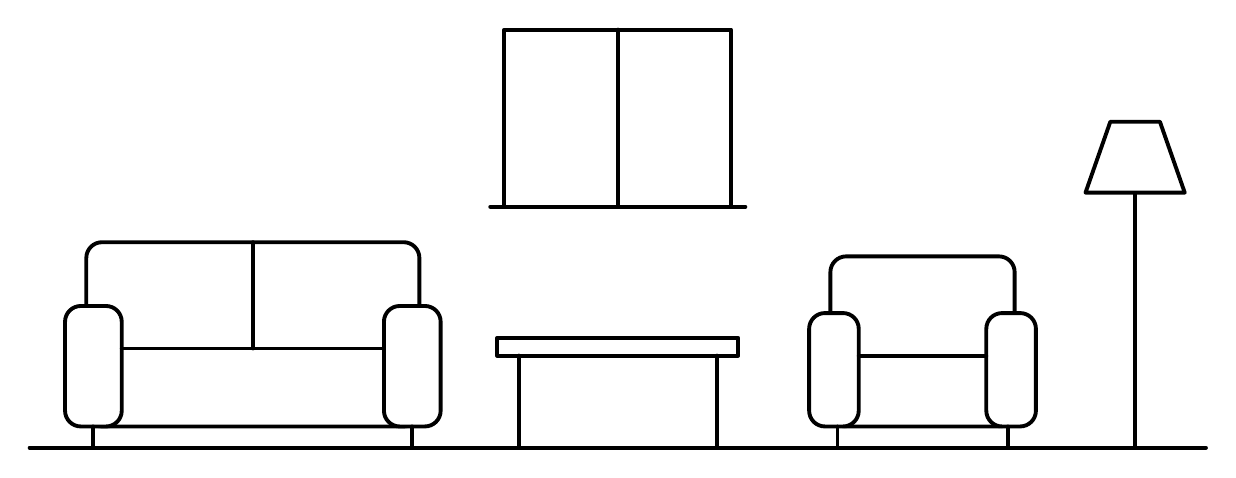
\begin{tikzpicture}[line width=1.4pt, line cap=round, line join=round, scale=0.9]
  \draw (-0.3,0) -- (16.3,0);
  % la ventana
  \filldraw[fill=white] (6.4,3.4) rectangle (9.6,5.9);
  \draw (8.0,3.4) -- (8.0,5.9); \draw (6.2,3.4) -- (9.8,3.4);
  % el sofá
  \filldraw[fill=white, rounded corners=2mm] (0.5,0.3) rectangle (5.2,2.9);
  \filldraw[fill=white, rounded corners=2mm] (0.2,0.3) rectangle (1.0,2.0);
  \filldraw[fill=white, rounded corners=2mm] (4.7,0.3) rectangle (5.5,2.0);
  \draw (1.0,1.4) -- (4.7,1.4); \draw (2.85,1.4) -- (2.85,2.9);
  \draw (0.6,0.3) -- (0.6,0); \draw (5.1,0.3) -- (5.1,0);
  % la mesita baja
  \filldraw[fill=white] (6.3,1.3) rectangle (9.7,1.55);
  \draw (6.6,1.3) -- (6.6,0); \draw (9.4,1.3) -- (9.4,0);
  % el sillón
  \filldraw[fill=white, rounded corners=2mm] (11.0,0.3) rectangle (13.6,2.7);
  \filldraw[fill=white, rounded corners=2mm] (10.7,0.3) rectangle (11.4,1.9);
  \filldraw[fill=white, rounded corners=2mm] (13.2,0.3) rectangle (13.9,1.9);
  \draw (11.4,1.3) -- (13.2,1.3);
  \draw (11.1,0.3) -- (11.1,0); \draw (13.5,0.3) -- (13.5,0);
  % la lámpara de pie
  \draw (15.3,0) -- (15.3,3.6); \draw (14.8,0) -- (15.8,0);
  \filldraw[fill=white] (14.6,3.6) -- (16.0,3.6) -- (15.65,4.6) -- (14.95,4.6) -- cycle;
\end{tikzpicture}
